\section{Problem Statement}
\label{sec:intro}

In part due to public policy, the average levels of fine particulate matter (PM\textsubscript{2.5}) in the US have generally been declining over the past few decades \cite{clean_air_act}. Despite those improvements, the contribution of wildfire smoke to PM\textsubscript{2.5} concentrations in the US has been calculated to have more than doubled between 2010 to 2020, accounting for up to half of the overall PM\textsubscript{2.5} exposure in Western regions \cite{smoke_PM}. Increases in PM\textsubscript{2.5} due to wildfire smoke are concerning since ambient PM\textsubscript{2.5} exposure is a leading environmental risk factor for adverse health effects and premature mortality \cite{smoke_mortality}.  These risks underscore the necessity for efficient and effective monitoring methods to mitigate the adverse health impacts associated with wildfire smoke. 

Satellite imagery, equipped with state-of-the-art sensors, such as the Advanced Baseline Imager (ABI) on the Geostationary Operational Environmental Satellites (GOES) \cite{goes}, have revolutionized environmental monitoring. Compared to orbiting satellites such as the Suomi or Sentinel satellites, geostationary satellites maintain constant observation over a fixed area. GOES offers the advantage being able to reliably and consistently capture the dynamic behavior of wildfire smoke plumes. In turn, GOES capabilities can provide critical insights into the concentration and movement of smoke particulates, facilitating real-time assessments of air quality.

Current fire detection algorithms rely primarily on calculating the fire radiative power (FRP) of active fires using near-infrared (NIR) satellite bands \cite{frp}. When fires have thick smoke plumes, the smoke can obfuscate a satellite's view of an active fire, making FRP impossible to calculate. If combined with FRP calculations, a real-time widlfire smoke plume analysis product can deliver additional insight into an active wildfire's activity level. 

Generally, integrating satellite imagery into wildfire smoke monitoring provides real-time data that can improve the timeliness of public health planning and response. By mapping the spread and density of smoke, health authorities can issue prompt warnings, implement evacuation protocols, and deploy resources effectively to mitigate health risks. Furthermore, long-term data gathered from satellite observations can aid in understanding the broader impacts of wildfire smoke on public health, influencing policy decisions and preventive measures. 

To address the need for a timely smoke analysis product, we present SmokeViz, an ensemble based deep learning method to identify and classify smoke plumes in satellite imagery. The model is a result of a successful project at the Global Systems Laboratory at the National Oceanic and Atmospheric Administration (NOAA) to build a large scale dataset of smoke plumes in GOES imagery. Keeping in mind the correlation between both the quality and quantity of data with deep learning model performance, we introduced the largest known smoke plume dataset, containing over 180,000 samples. The resulting dataset was used to train an ensemble of deep learning models that decorrelate errors by varying the inductive biases and give a more robust prediction than any singular model. 

We propose bringing SmokeViz to NOAA's Fire Weather Testbed to evaluate it's capabilities to (1) replace or enchance NOAA's current human annotated smoke product and (2) improve latency in NOAA's smoke dispersion models by using it as a smoke analysis product. The following subsections elaborate on the current needs for SmokeViz in these two application areas. 

\subsection{Replacing the Hazard Mapping Systems Smoke Product} 

\begin{figure*}
    \centering
    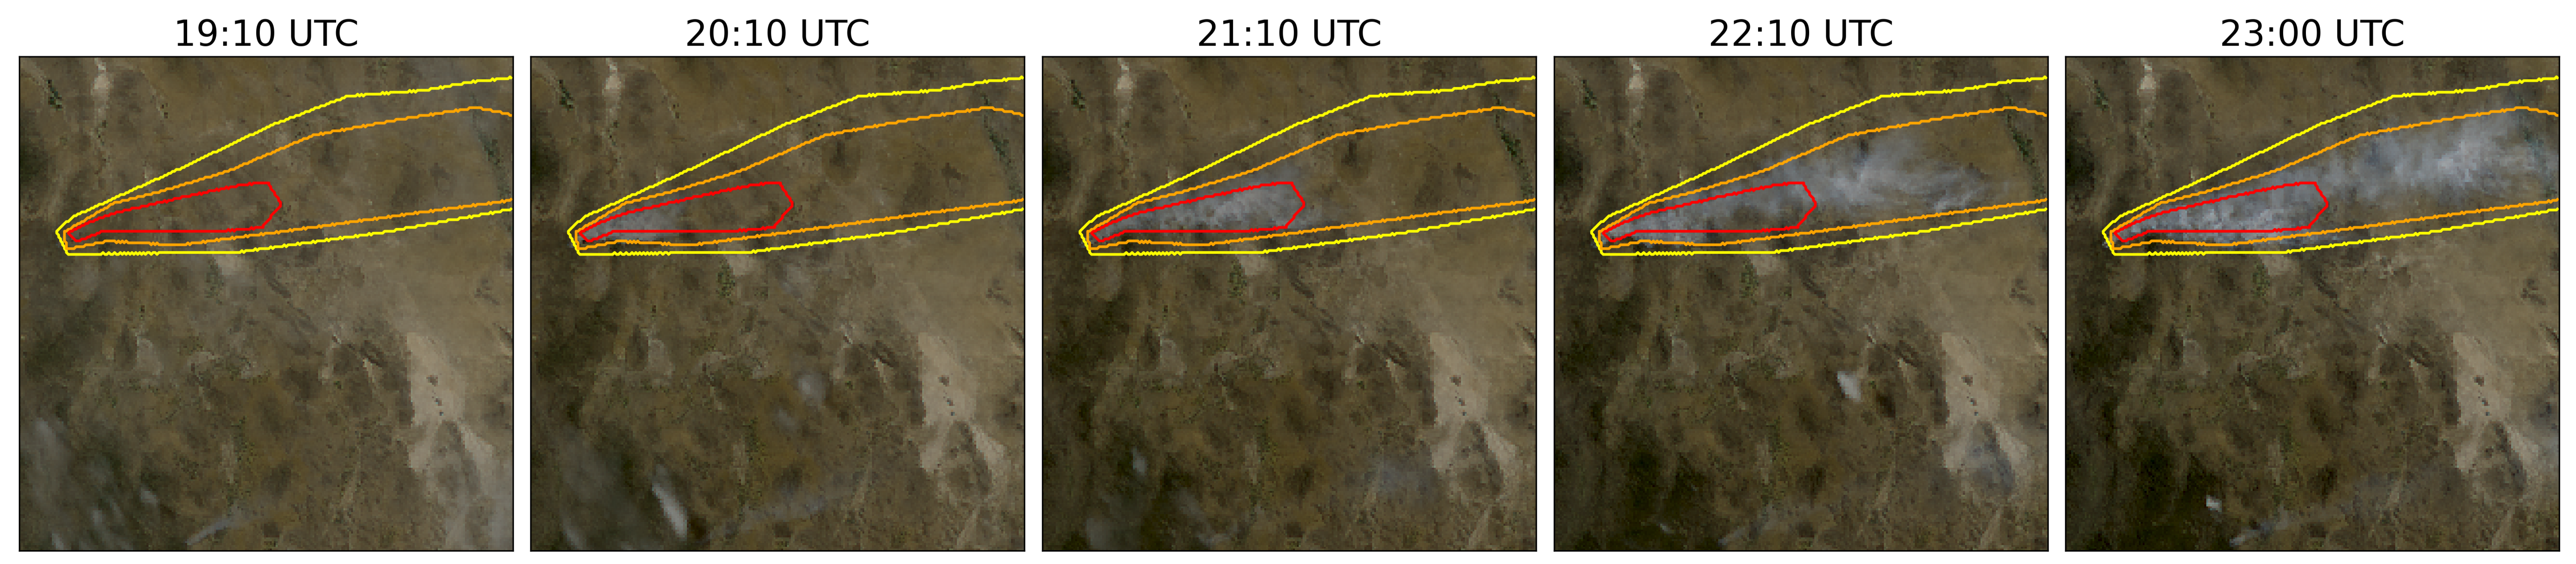
\includegraphics[width=\linewidth]{figures/TIMELAPSE_FINAL2.png}
    \caption{True color GOES-East imagery from May 5th, 2022, Southeast New Mexico (\(31.38^{\circ}\)N, \(107.87^{\circ}\)W) during the start of the Foster Fire. The red, orange and yellow lines represent the heavy, medium and low density HMS smoke annotations that span 19:10\textendash23:00 UTC.}
    \label{timelapse}
\end{figure*}

The National Oceanic and Atmospheric Administration (NOAA) manages environmental satlelite programs such as the Hazard Mapping System (HMS) program that uses an aggregation of satellite data to generate active fire and smoke data \cite{hms, hms_val}. The HMS smoke product \cite{hms, hms_val} is generated by human visual inspection of GOES satellite imagery for smoke identification. Trained satellite analysts use movement characteristics to help identify smoke by scanning through a time series of satellite images. When visual inspection indicates smoke, the analyst will draw a polygon that corresponds to the geolocation and density of smoke. HMS smoke analysis data gives the coordinates of the smoke perimeter as a polygon and classifies the smoke by density within a given time window. The time windows can range from instantaneous (same start/end time) to lengths of 22 hours, with an average time window around 3 hours. While the true bounds of the smoke can change within the larger time spans (figure \ref{timelapse}), the analyst is making an approximation that should reflect the smoke coverage over the duration of the time window. The density information is qualitatively determined by each analyst based on the apparent smoke opacity in the satellite imagery and categorized as either light, medium or heavy as seen in figure \ref{densities}a \cite{hms_web}. The HMS smoke product is released on a rolling but undefined schedule ranging from one to multiple times a day as observation conditions permit and is heavily limited by the availability of analysts and their time. 

Due the primarily its coarse time resolution and latency between the event and the corresponding annotation, the HMS smoke product is not an ideal candidate for a smoke analysis product for real-time smoke dispersion forecasting. Current end users of the HMS smoke product include the Environmental Protection Agency's AirNow program, NOAA's hurricane center and Mexico's National Weather Service. SmokeViz offers the current capabilities with additional advancements to the HMS product, some of the immediate items of improvement include higher time resolution and real-time analysis on streaming GOES data. 

Additionally, through the fire weather testbed, we aim to verify that SmokeViz is able to provide more consistency in smoke density labels, better detail of smoke borders and detect smoke plumes missed by analysts. 

\begin{figure*}
    \centering
    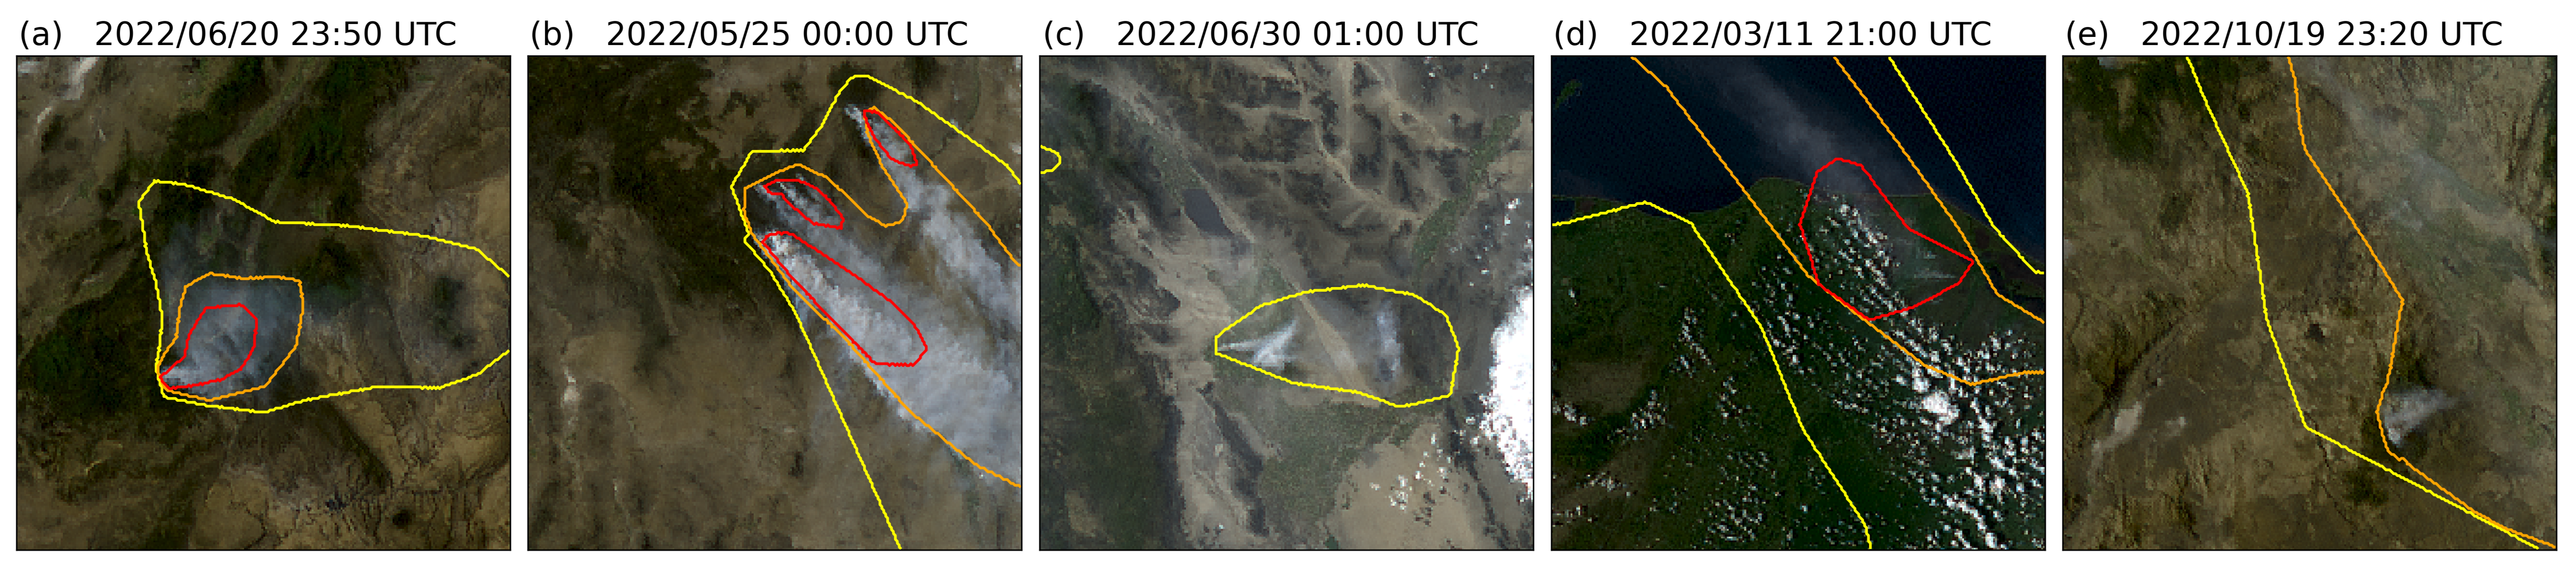
\includegraphics[width=\linewidth]{figures/variations2.png}
    \caption{HMS smoke annotations overlaid on GOES imagery, the yellow, orange and red contours indicate the extent of light, medium and heavy density smoke. (a) and (b) show a canonical examples of a smoke plumes. (c)-(e) show observable variations in the density labels.}\label{densities}
\end{figure*}


\subsection{Introducing a Smoke Analysis Product for Data Assimilation}

The High-Resolution Rapid Refresh (HRRR) model and prototype Rapid Refresh Forecast System (RRFS) produce short-range weather forecasts for CONUS and Alaska, including predictions of wildfire smoke. For each hour, the model is initialized using meteorological data assimilation, combining weather observations with a 3-D model background. While these models use satellite-detected FRP to determine location and smoke emissions associated with wildfires, there is currently no assimilation of smoke observations. We propose to use a deep learning derived smoke identification product to create a smoke analysis to initialize HRRR or RRFS.  

Currently, HRRR and RRFS have a significant latency for representing the plumes from recently started wildfires figure \ref{marshall}.  HRRR relies on polar-orbiting satellites, which only pass over a point on Earth’s surface twice per day.  RRFS uses detections from geostationary satellites, which can detect fires with much lower latency, but depends on the Regional ABI and VIIRS fire Emissions (RAVE) algorithm which takes some time to run.  In addition, formal data assimilation of either satellite aerosol optical depth (AOD) or surface-based smoke observations takes considerable computational time and resources.  For these reasons, a deep learning based smoke analysis could significantly improve short-range model forecasts in rapidly evolving situations featuring new fire starts.  

\begin{figure*}
    \centering
    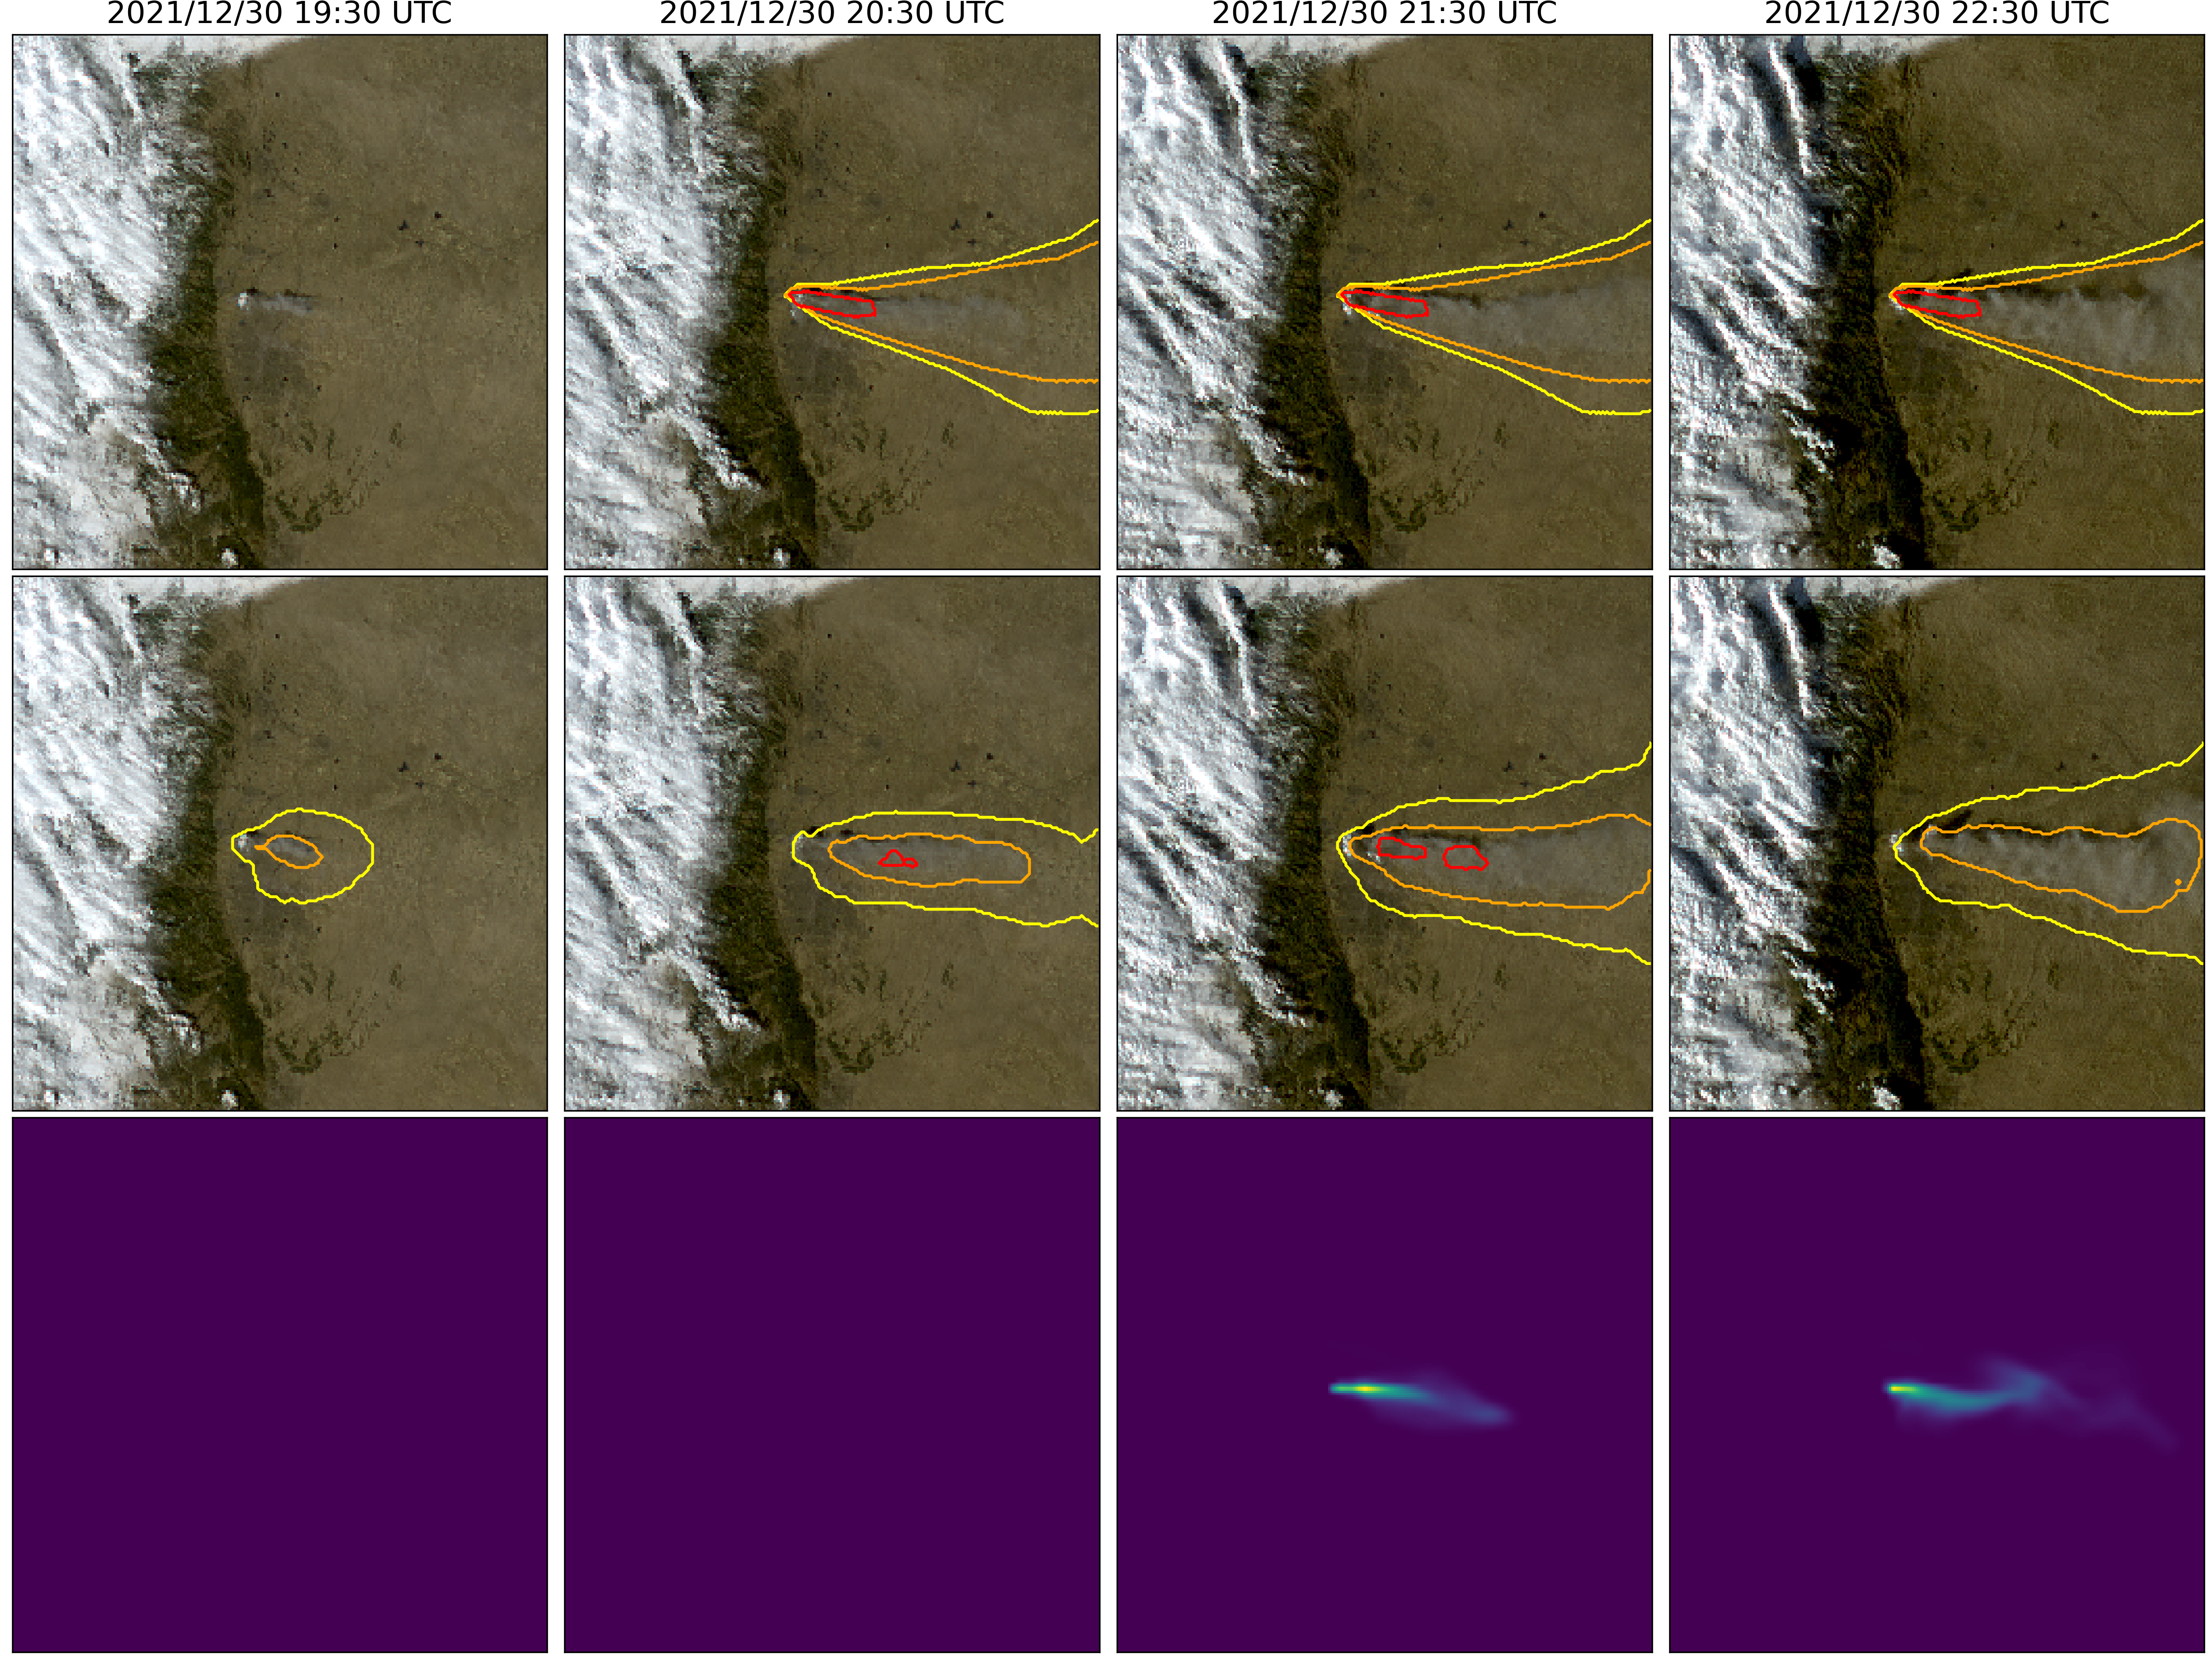
\includegraphics[width=\linewidth]{figures/marshall.png}
    \caption{Top row shows the HMS smoke annotations, middle is SmokeViz and bottom row is HRRR smoke for the start of the Marshall fire in Boulder, CO on December 29th, 2021.}\label{marshall}
\end{figure*}

\section{Methods and Activities}

While we will work directly with the fire weather testbed to develop a thorough and fair proccess for SmokeViz evaluation, here we will provide a summary of key aspects we will address.

\begin{equation} \label{overall_iou}
    IoU_{\text{overall}} = \frac{\sum\limits_{i=\text{light}}^{\text{heavy}}|y_{i}\cap y^*_{i}|}{\sum\limits_{i=\text{light}}^{\text{heavy}}|y_{i}|\cup|y^*_{i}|}
\end{equation}

\begin{figure*}
    \centering
    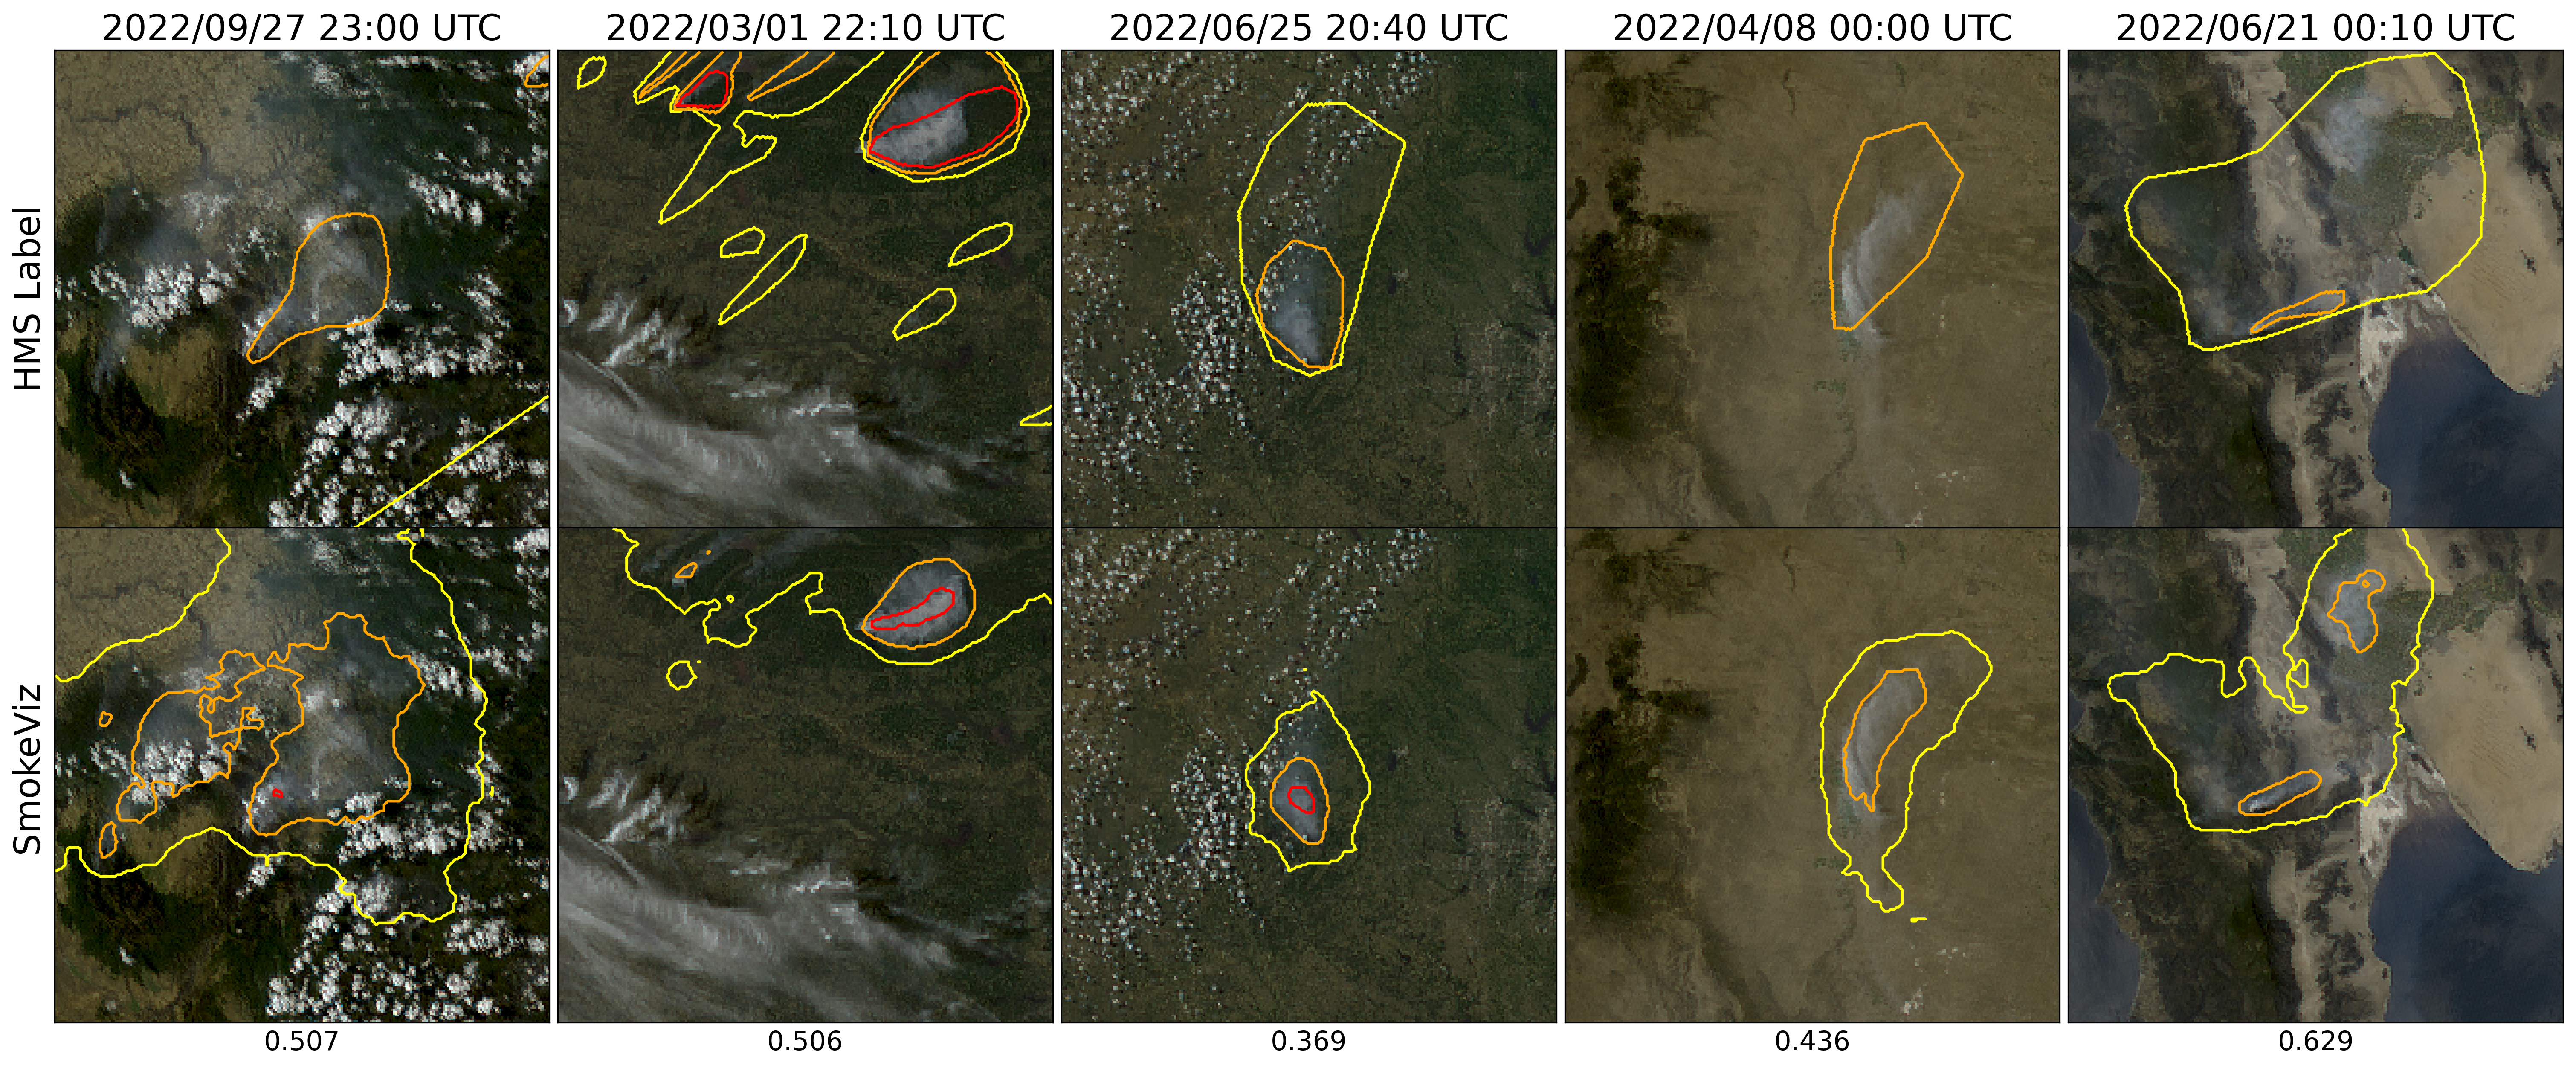
\includegraphics[width=17cm]{figures/examples.png}
    \caption{Examples of HMS annotations (top row) vs SmokeViz model output (bottom row) on SmokeViz dataset samples. The overall IoU score is reported at the bottom of each column.}\label{examples}
\end{figure*}

\begin{enumerate}
    \item \textbf{Identify all the relevant end users.} We have the HMS analysts that would directly use the product and HRRR/RRFS smoke dispersion model developers, but would want to determine if including further down the line users would be relevant to the evaluation. The HMS smoke product and HRRR forecast is publically published online so that it is difficult to track all users, but we will develop a strategy for identifying and communicating with users.

    \item \textbf{Establish the needs for all end users.} While we have the needs established for those end users that are collaborators on this proposal, we need to perform an assessment on current further down the line end users of the HMS smoke product.

    \item \textbf{Survey how to improve training material and documentation.} We have a tutorial available on how to use the SmokeViz model on specified GOES imagery, but would want to do further assessments on how we can make it more user-friendly to not only the scientific community but also the general public. This would be an iterative proccess that would start before the official testbed evaluation event. Success of the training materials will be included as part of the testbed evaluation.


\item \textbf{Determine evaluation metrics.} 

    \item \textbf{Develop evaluation scenarios.} The SmokeViz model was trained on smoke plumes from 2018-2021 and 2024. 2023 data served to validate the model and 2022 was used for final performance testing. Since neither of those years were used for training the model they could be included for testbed evaluation but it would be important to add in events from 2025 that the model has never touched before. We would need to include scenarios from varying solar zenith angles during the day and over different seasons of the year. Since the SmokeViz model domain covers all of North America, there should be scenarios that span multiple geolocations within those boundaries. While currently untested, we anticipate SmokeViz to have similar performance in the Southern hemisphere and would include samples to test that hypothesis.

    \item \textbf{Perform evaluation.} 

\end{enumerate}


\section{Products/Outputs}
The project will produce an operationally-ready smoke analysis product that can be used for near-realtime DA for air quality models. Additionally, a comprehensive report on the operational utility of the SmokeViz product will be delivered in order to support operational deployment.

Potential end-user adopters of the SmokeViz product would include the scientists that create and run the air quality and smoke plume dispersion models along with down-the-line air quality forecasters and decision makers.

\section{Impacts/Benefits/Outcomes}

The expected result will be an efficient deep learning based smoke analysis product that describes the current extent and categorical density of smoke. Used as a smoke DA product, SmokeViz is expected to significantly advance short-range model predictive capabilities for rapidly evolving wildfires.

\section{Schedule}

\begin{tabular}{ |p{3cm}|p{3cm}|p{8cm}|  }
 \hline
 \multicolumn{3}{|c|}{Schedule} \\
 \hline
 Date & Start RL & milestone\\
 \hline
 Q1 & 5 & \\
 Aland Islands&   AX  & ALA   \\
 \hline
\end{tabular}

The current RL for this project is RL 5 where we have performed evaluation and testing for SmokeViz on streaming GOES imagery. At the end of this project timeline, we will work with a transition partner to reach readiness level 8.

\section{Outreach and Education}

We've developed a series of Jupyter Lab notebooks that walk users through the SmokeViz dataset hosted by NOAA on AWS that includes HMS analyst annotations and the corresponding GOES imagery. The notebooks demonstrate how the user can interact with the currated dataset to train their own deep learning models and how to apply the tested SmokeViz model to incoming GOES imagery in order to detect active smoke plumes.

The SmokeViz dataset and model serve as an excellent benchmark for learning how to work with large environmental datasets and deep learning models. We've put a lot of thought and effort into the reproducibility of the research along with readibility of the code and tools. Not only can users use the codebase for smoke plume realted projects but also as a toolkit for other remote sensing work involving satellite imagery and geospatial shape files. 

This proposal is focused on getting SmokeViz operational in the United States for detecting and monitoring wildfires in North America. We will reach out to facilitate virtual participation from Mexico's National Weather Service for the SmokeViz evaluation. Verification of SmokeViz for North America will give insights on developing additional deep learning wildfire smoke algorithms for other parts of the world that may not have the required resources to have analysts constantly monitor smoke plumes.


\section{Diversity and Inclusion}

The original SmokeViz dataset and model project began during the 2022 NOAA/CIRES summer internship program. This program was a CIRES diversity and inclusion initiative to give underrepresented graduate students opportunities to work with NOAA scientists. As a member of multiple underrepresented groups in the scientific community, PI Rey Koki was able to develop collaborations for SmokeViz directly through that internship opportunity. Since the end of that internship, Rey has since been hired as a CIRES research associate and continues work with SmokeViz and related projects at NOAA. Rey Koki identifies as queer, is half Pacific Islander and is the only member in their direct or extended family to hold a 4-year college degree, yet alone a graduate degree. 
 
Having a direct understanding of how fostering equity in science benefits the scientific community as a whole, Rey Koki is committed to continued efforts towards equity-centered approaches in their work. Related to this project, Rey Koki and collaborator Jebb Stewart developed an internship project with SmokeViz, where they mentored a summer 2024 Hollings undergraduate intern, Annabel Wade, who successfully implemented ensembling methods for SmokeViz. Rey Koki and Jebb Stewart continue to make efforts to facilitate research opportunities for students to gain experience working with SmokeViz.

\section{Data and/or Software Management Plan}

%-------------------------------------------------------------------------

